\section{Décomposition en produits}

\subsection{Approche organisationnelle}
L'organisation de l'équipe a été détaillée plus tôt.

\subsection{Approche produit}

Le système peut être décomposé en sous-système suivant le diagramme
présenté en figure 1.\\

\begin{figure}
\rotatebox{90}{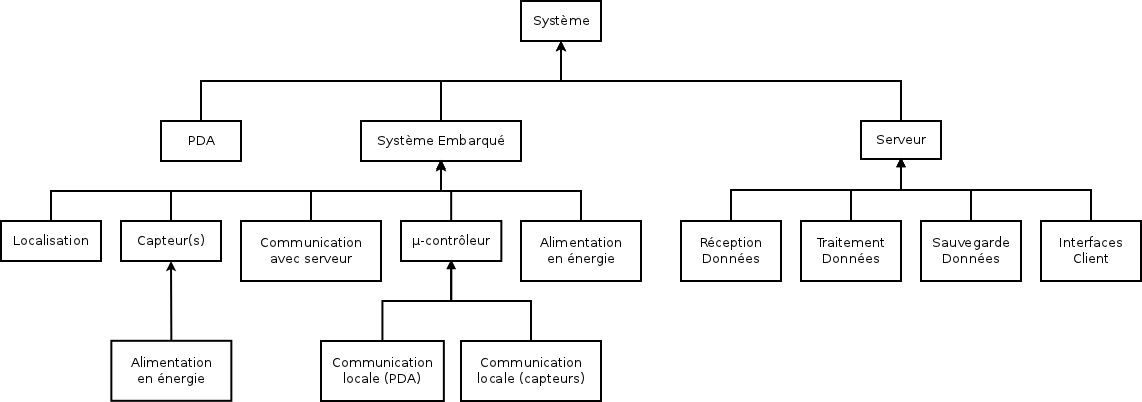
\includegraphics[scale=0.5]{\PIXPATH/decoupe1}
\end{figure}

Cela nous amène à dégager les sous-projets suivant :

\begin{itemize}
\item Conception matérielle du système embarqué
\item Programmation du système embarqué
\item Applicatif PDA
\item Intégration des différents sous-projets système
\item Gestion de la documention du projet
\item Formation des futurs utilisateurs
\end{itemize}


\subsection{Cycle de vie du système}

Ce projet sera découpé en plusieurs lots et plusieurs phases.
